\section{Spektrum Gelombang}
\label{sec:spektrum-gelombang}

Gelombang laut merupakan fenomena alam yang memiliki dua sisi berbeda - dapat tampil sebagai pemandangan yang memesona di satu waktu, namun juga bisa menjadi kekuatan yang mengancam di waktu lain. Pembentukan gelombang di laut umumnya dipicu oleh aktivitas angin. Prosesnya dimulai ketika angin berkecepatan rendah menciptakan riak-riak kecil \emph{(ripple)} di permukaan air. Seiring dengan peningkatan kecepatan angin dan hembusan yang berkelanjutan, riak-riak ini berkembang menjadi gelombang kecil, yang kemudian bergabung satu sama lain melalui proses superposisi hingga akhirnya membentuk gelombang yang lebih besar.

Secara matematis, gelombang laut dapat dijelaskan dengan cara yang mirip dengan sinyal acak dalam bidang elektronika atau getaran periodik pada sistem mekanis. Fenomena yang dikenal sebagai proses acak ini umumnya dapat direpresentasikan menggunakan deret Fourier, yang terdiri atas komponen-komponen periodik dengan frekuensi yang merupakan kelipatan dari frekuensi dasar \citep{Djatmiko_2012}.

\subsection{Analisis Fourier}
\label{subsec:analisis-fourier}

Secara matematis gelombang laut dapat dijelaskan sebagaimana halnya dengan sinyal acak di bidang elektronika ataupun getaran sistem periodis dalam sistem mekanika \citep{Djatmiko_2012}. Kondisi yang secara umum disebut sebagai proses acak tersebut dapat direpresentasikan oleh deret Fourier yang memuat komponen-komponen periodis dengan frekuensi-frekuensi yang merupakan multiplikasi dari frekuensi dasar $\omega$. Menurut referensi tersebut elevasi gelombang acak dapat dituliskan dalam bentuk persamaan:

\begin{equation}
\zeta(t) = \bar{\zeta} + \sum_{n=1}^{\infty} A_n\cos(\omega_nt) + B_n\sin(\omega_nt)
\label{eq:acak1}
\end{equation}

di mana komponen-komponen frekuensi tersebut adalah:

\begin{equation}
\omega_n = \frac{2\pi n}{T_R} \text{ (rad/det) untuk } n = 1,2,3,\ldots,\infty
\label{eq:acak2}
\end{equation}

dengan $T_R$ sebagai rentang waktu keseluruhan proses. $A_n$ dan $B_n$ adalah koefisien-koefisien yang dapat diberikan dalam bentuk persamaan:

\begin{equation}
A_n = \frac{2}{T_R}\int_0^{T_R}\zeta(t)\cos(\omega_nt)dt
\label{eq:acak3}
\end{equation}

\begin{equation}
B_n = \frac{2}{T_R}\int_0^{T_R}\zeta(t)\sin(\omega_nt)dt
\label{eq:acak4}
\end{equation}

Dengan demikian pers. \eqref{eq:acak1} dapat dituliskan kembali dalam bentuk gabungan fungsi periodik berikut:

\begin{equation}
\zeta(t) = \bar{\zeta} + \sum_{n=1}^{\infty}\zeta_n\cos(\omega_nt + \epsilon_n)
\label{eq:acak5}
\end{equation}

dengan amplitudo sebesar:

\begin{equation}
\zeta_n = \sqrt{(A_n^2 + B_n^2)}
\label{eq:acak6}
\end{equation}

serta sudut fase sebesar:

\begin{equation}
\epsilon_n = \arctan(-B_n/A_n)
\label{eq:acak7}
\end{equation}

Persamaan \eqref{eq:acak1}, dan selanjutnya pers. \eqref{eq:acak5}, pada dasarnya menunjukkan bahwa gelombang acak adalah tersusun dari superposisi gelombang-gelombang reguler yang jumlah yang secara teoritis sebenarnya adalah tidak berhingga. Penerapan persamaan tersebut dalam bidang rekayasa perkapalan terkhusus dalam pembentukan gelombang dapat dilihat pada gambar \ref{fig:pembentukan-gelombang-acak}.

\begin{figure}[!ht]
    \centering
    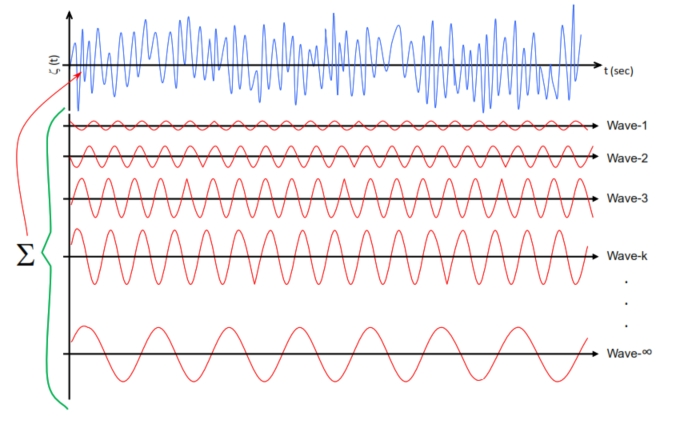
\includegraphics[width=0.7\textwidth]{gambar/pembentukan-gelombang-acak.jpg}
    \caption{Gelombang acak terbentuk dari superposisi gelombang-gelombang  reguler dalam jumlah tak berhingga}
    \label{fig:pembentukan-gelombang-acak}
\end{figure}

Pendekatan yang digunakan dalam menganalisis dan mengubah data gelombang menjadi spektrum energi merupakan adaptasi dari teknik yang umum digunakan dalam elektronika dan mekanika getaran. Inti dari proses ini adalah penggunaan deret Fourier untuk mentransformasikan data gelombang dari domain waktu ke domain frekuensi. Secara singkat proses pemodelan dimulai dengan mengambil data gelombang dari stasiun pengukuran kemudian dimodelkan dalam bentuk persamaan matematis dan dilakukan \emph{fitting} hingga persamaan yang dihasilkan mendekati hasil pengukuran. Hal ini menyebabkan keterbatasan keakuratan dan penggunaan setiap spektra gelombang. Berikut dijelaskan beberapa model spektra yang biasa digunakan.

\subsection{Bretschneider-1959}
\label{subsec:Bretschneider}

Formula spektra gelombang yang dipublikasikan oleh Bretschneider (1959) adalah merupakan spektra dengan dua paremeter, yakni tinggi gelombang signifikan $H_s$ dan frekuensi puncak spektra $\omega_0$. Persamaan ini sesuai untuk perairan terbuka, dan kondisi gelombang fully develop, dengan bentuk:

\begin{equation}
S_\zeta(\omega) = \frac{1.25 \omega_0^4}{4 \omega^5} H_s^2 \exp\left\{-1.25\left(\frac{\omega_0}{\omega}\right)^4\right\}
\label{eq:Bretschneider1}
\end{equation}

Frekuensi modal, atau frekuensi puncak spektra, dalam persamaan \eqref{eq:Bretschneider1} dapat diperoleh sebagai fungsi tinggi gelombang signifikan, sebagai berikut:

\begin{equation}
\omega_0 = \sqrt{0.161 g / H_s}
\end{equation}

\subsection{JONSWAP}
\label{JONSWAP}

JONSWAP adalah merupakan singkatan dari \textit{Joint North Sea Wave Project}, yakni proyek yang dilakukan secara bersama-sama oleh sejumlah negara untuk melakukan penelitian gelombang di perairan Laut Utara. Menurut laporan dari Hasselman dkk (1973, 1978) formulasi spektra JONSWAP adalah merupakan modifikasi dari spektra P-M, dengan memasukkan parameter-parameter yang akan mengakomodasi karakteristik gelombang perairan tertutup, atau kepulauan. Persamaan spektra JONSWAP mempunyai bentuk yang lebih kompleks bila dibandingkan dengan persamaan-persamaan spektra lain, sebagai berikut:

\begin{equation}
S_\zeta(\omega) = \alpha\omega^{-5} \exp\left\{-1.25(\omega/\omega_b)^{-4}\right\}\gamma^{\exp\left\{-\frac{(\omega-\omega_0)^2}{2\sigma^2\omega_0^2}\right\}}
\end{equation}

di mana:
\begin{align*}
\alpha &= 0.076(X_*)^{-0.22} \\
X_* &= gX/U_*^2 \\
X &= \text{panjang fetch} \\
U_* &= \text{kecepatan angin} \\
\alpha &= 0.0081 \text{ jika } X \text{ tidak diketahui} \\
\sigma &= \text{parameter kemiringan atau \textit{peakedness parameter}, yang harganya} \\
      &\text{  dapat bervariasi antara 1.0 sampai dengan 7.0. Untuk Laut Utara} \\
      &\text{  mempunyai harga 3.3} \\
\tau &= \text{parameter bentuk atau \textit{shape parameter}} \\
\tau &= 0.07 \text{ jika } \omega \leq \omega_0 \\
\tau &= 0.07 \text{ jika } \omega > \omega_0 \\
\tau &= 2g^2(X_*)^{-0.33}
\end{align*}

Formulasi spektra JONSWAP akhir-akhir ini banyak dipakai dalam perancangan dan analisis bangunan lepas pantai yang dioperasikan di Indonesia. Hal ini cukup dapat dimengerti karena perairan Indonesia di mana kebanyakan bangunan lepas pantai untuk kegiatan migas dioperasikan adalah merupakan perairan kepulauan atau perairan tertutup.